%% LyX 2.0.8.1 created this file.  For more info, see http://www.lyx.org/.
%% Do not edit unless you really know what you are doing.
\documentclass[10pt,landscape,british,pra,twocolumn,superscriptaddress,nofootinbib,nobibnotes,tightenlines,longbibliography]{revtex4}
%\bibliographystyle{aipnum4-1}
%\bibliographystyle{apsrev4-1}
%\usepackage{doi}

\bibliographystyle{plainnat}
\usepackage[T1]{fontenc}
\usepackage[latin9]{inputenc}
\pagestyle{plain}
\setcounter{secnumdepth}{3}
\usepackage{color}
\usepackage{refstyle}
\usepackage{amsmath}
\usepackage{amssymb}
\usepackage{graphicx}
\usepackage{esint}

\makeatletter

%-----------New commands (`Atul's')
\newcommand{\floor}[1]{\lfloor #1 \rfloor}
\newcommand{\ab}[1]{\left| #1 \right|}

%---------- New commands

%\usepackage{multicol}
\newcommand{\mean}[1]{\langle #1 \rangle}
\newcommand{\ket}[1]{| #1 \rangle}
\newcommand{\bra}[1]{\langle #1 |}
\newcommand{\rb}[1]{\left( #1 \right)}
\newcommand{\mb}[1]{\mathbf{#1}}
\newcommand{\ew}[1]{\langle #1 \rangle}
\newcommand{\beq}{\begin{eqnarray}}
\newcommand{\eeq}{\end{eqnarray}}
\newcommand{\blg}[1]{\mathrm{lg}\left[  #1right]}
\newcommand{\svec}{\mbox{\boldmath$\sigma$}}
\newcommand{\op}[2]{| #1 \rangle \langle #2 |}
\newcommand{\sech}{\mathrm{sech}}
\newcommand{\sfrac}[2]{\begin{array}{c}\frac{#1}{#2}\end{array}}
\newcommand{\cum}[1]{\langle\langle #1 \rangle \rangle}
\newcommand{\eq}[1]{Eq.~(\ref{#1})}
\newcommand{\fig}[1]{Fig.~\ref{#1}}
\newcommand{\ul}[1]{{\underline{#1}}}
\newcommand{\bs}[1]{\boldsymbol{#1}}
\newcommand{\trace}[1]{\mathrm{Tr}\left\{#1\right\}}

\newcommand{\etal}{{\em et al.}\xspace}

% Ali's commands
\newcommand{\proj}[1]{\ket{#1}\!\bra{#1}}


% GME vector notation
\newcommand{\kett}[1]{| #1 \rangle\!\rangle }
\newcommand{\braa}[1]{\langle\!\langle #1|}
\newcommand{\eww}[1]{\langle\! \langle #1\rangle\! \rangle}
\newcommand{\opp}[2]{| #1 \rangle\! \rangle\langle\! \langle #2 |}
\DeclareMathOperator{\tr}{tr}
\renewcommand\Re{\operatorname{Re }}
\renewcommand\Im{\operatorname{Im }}

% citation command Ref.[...]
\newcommand{\citer}[1]{{Ref.~\cite{#1}}}
\definecolor{mygray}{gray}{0.5}
\definecolor{mymagenta}{cmyk}{0,1,0,0.12}
\newcommand{\mtext}[1]{{\color{mymagenta}#1}}
\newcommand{\rtext}[1]{{\color{red} #1}}


%------------

%%%%%%%%%%%%%%%%%%%%%%%%%%%%%% LyX specific LaTeX commands.

\AtBeginDocument{\providecommand\subref[1]{\ref{sub:#1}}}
\AtBeginDocument{\providecommand\figref[1]{\ref{fig:#1}}}
\pdfpageheight\paperheight
\pdfpagewidth\paperwidth

%% Because html converters don't know tabularnewline
\providecommand{\tabularnewline}{\\}
%% A simple dot to overcome graphicx limitations
\newcommand{\lyxdot}{.}

\RS@ifundefined{subref}
  {\def\RSsubtxt{section~}\newref{sub}{name = \RSsubtxt}}
  {}
\RS@ifundefined{thmref}
  {\def\RSthmtxt{theorem~}\newref{thm}{name = \RSthmtxt}}
  {}
\RS@ifundefined{lemref}
  {\def\RSlemtxt{lemma~}\newref{lem}{name = \RSlemtxt}}
  {}


%%%%%%%%%%%%%%%%%%%%%%%%%%%%%% Textclass specific LaTeX commands.
\@ifundefined{textcolor}{}
{%
 \definecolor{BLACK}{gray}{0}
 \definecolor{WHITE}{gray}{1}
 \definecolor{RED}{rgb}{1,0,0}
 \definecolor{GREEN}{rgb}{0,1,0}
 \definecolor{BLUE}{rgb}{0,0,1}
 \definecolor{CYAN}{cmyk}{1,0,0,0}
 \definecolor{MAGENTA}{cmyk}{0,1,0,0}
 \definecolor{YELLOW}{cmyk}{0,0,1,0}
}
\newenvironment{lyxlist}[1]
{\begin{list}{}
{\settowidth{\labelwidth}{#1}
 \setlength{\leftmargin}{\labelwidth}
 \addtolength{\leftmargin}{\labelsep}
 \renewcommand{\makelabel}[1]{##1\hfil}}}
{\end{list}}

%%%%%%%%%%%%%%%%%%%%%%%%%%%%%% User specified LaTeX commands.
%\renewcommand*{\thefootnote}{\fnsymbol{footnote}}
%%\renewcommand*{\thefootnote}{\arabic{footnote}}
%\setcounter{footnote}{0}
%\usepackage{perpage} %the perpage package
%\MakePerPage{footnote} %the perpage package command
\usepackage{cancel}
\usepackage{braket}
\usepackage{tikz}

\newcommand{\Plus}{\mathord{\begin{tikzpicture}[baseline=0ex, line width=1, scale=0.13]
\draw (1,0) -- (1,2);
\draw (0,1) -- (2,1);
\end{tikzpicture}}}

\newcommand{\Minus}{\mathord{\begin{tikzpicture}[baseline=0ex, line width=1, scale=0.13]
\draw (0,1) -- (2,1);
\end{tikzpicture}}}


%\newcommand{\Plus}{\mathord{\tikz\draw[line width=0.3ex, x=1ex, y=1ex] (0.5,0) -- (0.5,1)(0,0.5) -- (1,0.5);}}
%\newcommand{\Minus}{\mathord{\tikz\draw[line width=0.3ex, x=1ex, y=1ex] (0,0.5) -- (1,0.5);}}

\makeatother

\usepackage{babel}

\begin{document}

\title{Towards macroscopic Bell test with modular variables}


\author{Atul Singh Arora}


\address{University of Siegen, Germany}


\address{Indian Institute of Science Education \& Research, Mohali, India}


\author{Ali Asadian}


\address{University of Siegen, Germany}


\pacs{Draft}


\date{May-July 2015}
\begin{abstract}
We propose local realism tests demonstrated by correlation measurements of  continuum valued function of position and momentum variables, known as modular variables. These observables are described by bounded function in Wigner representation of phase sapce, and therefore,  the associated inequality holds for any state described by positive Wigner function. This conform with Bell's remark that positive Wigner function serving as a valid probability distribution never reveal nonlocality. We construct a class of entangled states leading to the violation of the inequality, and thus truly demonstrate nonlocality in phase space. The states can be realized in interferometric setups though grating techniques. The nonlocality is verified from spatial correlation data detected from the screens.
\end{abstract}
\maketitle

\section{Introduction}


In 1935, Einstein, Podolsky, and Rosen 
argued in a thought experiment that the quantum-mechanical description of 
physical reality is not complete, and thus may be superseded by a more 
complete realistic theory which reproduces the quantum mechanical predictions, and 
at the same time, obeys the locality condition \cite{EPR}. In his groundbreaking paper in 1964 \cite{Bell}  
Bell derived an experimentally testable inequality, which
bounds the correlations between bipartite measurements
for any such local hidden-variable theory, but which is violated
by quantum mechanics. This was a major breakthrough towards empirical 
tests of quantum mechanics as apposed to common sense theories. Since 
then, the results constraining the permissible types of hidden variable 
models of quantum mechanics have attracted much attention and have been 
reformulated as the problem of contextual measurements by Kochen and 
Specker~\cite{Kochen} and in terms of temporal correlations by Leggett 
and Garg~\cite{LG85}. Today, these concepts have mainly been formulated for intrinsic quantum degree of freedom of microscopic particles such as spins, and tested in various 
experiments with photons~\cite{Aspect1999}, ions~\cite{Roos09}, impurity spins~\cite{WaldherrPRL2011,KneeNatComm2012} or superconducting 
qubits~\cite{Palacios-LaloyNatPhys2010}. All experimental observations confirmed the validity of quantum nonlocality on this level. 
 
The outstanding challenge is, however, to formulate similar tests with truly spatial degree of freedom and observe the nonlocality directly from the observation of phase space coordinates. This can be considered as a natural extension to macroscopic limit of local realism tests [ ]. Moreover, phase space is a natural concept in classical theory and it is equivalent to the state space. This come along with the original EPR argument which uses phase space descriptions to better address the reality and locality problems of quantum mechanics in such manifold. Notably, the Wigner function associated with the entangled state used in EPR argument, so called EPR state, is positive every where. That is why, Bell argued that EPR states  do not lead to violation of the inequalities derived from
local hidden variable assumptions. Because, positive Wigner functions serve as valid joint probability distributions over local \emph{hidden} positions and momenta. Thereby, such state are compatible with a model of local hidden variable description. Banaszek and Wodkiewicz, however, showed that using particular measurements, Parity measurements, EPR states can reveal nonlocal feature indicating that not only the state itself but the type of correlation measurements is also important in any local realism tests. This opens the discussion as to   The problem of constructing a ``macroscopic'' test of local hidden variable models lies in choocing  proper observables whose  Wigner representations satisfy the constraint imposed by the algebraic CHSH expression. Throughout the paper, we will use the term ``macroscopic'' to refer to measurements of particles' phase space coordinates.




The paper is organized as follows.
In Sec. we introduce our framework for Bell nonlocality test aiming to use most classical-like variables and measurements, and thus pave the way towards macroscopic test of local realism.  In Sec. We present an explicit example by constructing a modular variable Bell operator for which the violation achieve if and only if the state described by negative Wigner function. In Sec. we proceed with identifying the relevant entangled state leading to the violation of the Bell inequality. Finally, in Sec. we propose a possible implementation of the desired entangled states




\section{Framework for macroscopic Bell test}

In what follow we develop a new test of local realism which comply with above Bell's argument.
The central 
problem here is to construct a Bell-operator of the Clauser-HorneShimony-Holt (CHSH) form
\[
\label{Bellmodular}
\hat {\mathcal{B}} \equiv \hat A_1\otimes (\hat A_2+\hat A_2') +\hat A_1'\otimes(\hat A_2-\hat A_2')
\]
expressed in terms of suitable local continuous variable (CV) observables $\hat A$ taking on a limited range of values to be able to determine a well-defined classical bound. We therefore aim to construct a class of bounded observables of CV systems which have the following properties. Using proper rescaling for corresponding quantum eigenvalues of the observable we have $
|a_j|\leq 1$.
One obvious example is parity operator which used in Ref [ ]. This is enough to construct a valid Bell operator with a well-defined classical bound. We however demand of an extra constraint required for probing Nonlocality in phase space. We impose that the observable $\hat A$ corresponds to a bounded c-number function in phase space using Wigner-Weyl correspondence ($q\leftrightarrow \hat q$, $p\leftrightarrow \hat p$). That is, 
\[
\mathcal{W}_{\hat A}(q, p) \equiv \int dq' e^{ipq'}\bra{q-\dfrac{q'}{2}}\hat A \ket{q+\dfrac{q'}{2}}\leq 1
\] 
Therefore,
\begin{align*}
\mathcal{W}_{\hat {\mathcal{B}}}(\bs q,\bs p)&=\mathcal{W}_{\hat A_1}(q_1,p_1)[\mathcal{W}_{\hat A_2}(q_2,p_2)+\mathcal{W}_{\hat A_2'}(q_2,p_2)] \\&+\mathcal{W}_{\hat A'_1}(q_1,p_1)[\mathcal{W}_{\hat A_2}(q_2,p_2)-\mathcal{W}_{\hat A_2'}(q_2,p_2)]\leq 2
\end{align*}
where $\bs q=(q_1,q_2)$ and  $\bs p=(p_1, p_2)$. Accordingly, the inequality should hold for any state described by valid (positive) probability distribution over phase space.
Therefore,
\begin{equation}
\mean{\hat{\mathcal{B}}}=\int W_{\hat {\rho}}(\bs q,\bs p)\mathcal{W}_{\hat {\mathcal{B}}}(\bs q,\bs p)d\bs q d\bs p\leq 2
\end{equation}
where $W_{\hat{\rho}}$ is the Wigner quasi-probability distribution corresponding to $\hat {\rho}$ given by $
W_{\hat {\rho}} = \mathcal{W}_{\hat {\rho}}/2\pi \hbar$. Parity operators do not fulfill above requirement. Because the corresponding Wigner representation of them are given by delta functions which are unbounded in phase space. This already voids the above inequality. With this, we ascertain that any state described by positive definite Wigner function, including EPR states, satisfy above class of Bell inequality. Hence, any state  leading to violation must be characterized by negative Wigner function deviating from proper probability distribution for (hidden) phase space coordinates. 

%That's why,  John Bell remarked that as EPR state described by positive Wigner function is compatible with a local hidden variable model, and thus it does not demonstrate nonlocality. This claim can be justified in the sense of above.
 
It is well recognized and it can be shown that .. that there is a tight relation between nonlocality and noncommutativity of operators. The violation occurs for choices of settings whose corresponding observable do not commute. It would be interesting the framework for the Bell test clearly demonstrates that the source of the violation directly originates from the noncommutativity  of the phase space quadratures in quantum mechanics, $[q,p]=i\hbar$. For macroscopic test the measurement scheme used for evaluating the correlations should have a classical analog for better understanding the result in classical limit. The parity operator measurements are defined in terms of resolving the  consecutive eigen values  with no classical analog. Therefore we do not consider it as ``classical-like'' measurement.

\subsection{Phase space translation operators and modular variables }

One particular class of bounded observable can be constructed from the quantum mechanical space translation operator\footnote{Here $-L/\hbar$ causes a displacement by $L$.}, $e^{-i\hat p L/\hbar}$. This observable is not hermitian and therefore it does not correspond to an observable. We define
\begin{align}
\begin{split}
  \label{translation}
  \hat X \equiv \text{Re}(e^{-i\hat p L/\hbar})&=(e^{-i\hat p L/\hbar}+e^{i\hat p L/\hbar})/2 \\ &=\cos(\hat p L/\hbar)
\end{split}
\end{align}
which is not only explicitly hermitian and $\le 1$, in fact the corresponding real function $\mathcal W_{\hat X}=\cos(pL/\hbar)$ is also manifestly  $\le 1$. In addition, there're three relavent properties. First, from equation \ref{translation}, the action of $\hat X$ is obvious. This entails that spatial symmetry must be harnessed to construct the appropriate entangled state. Second, when $\hat X$ is operated on $\ket{p}$, then only the modular part of $p$ is relevant to the value of the operator. Thus we may define 
\[
\hat p_{\text{mod}}\equiv \int dp \, p\text{mod}{h/L} \ket{p}\bra{p}
\]
and note that measuring $\hat p_{\text{mod}}$ is sufficient for obtaining the value of $\hat X$. Conversely, measuring $\hat X$ only yields $\hat p_{\text{mod}}$, not $\hat p$.
And finally, we could define an anlogous momentum translation operator and obtain the following relation
\[
e^{i\hat{p}u}e^{i\hat{q}v}=e^{i\hbar uv}e^{i\hat{q}v}e^{i\hat{p}u}
\]
using $[q,p]=i\hbar$. For appropriate choices of $u,v$, the translation operators can be made to commute or anti-commute. In the former case, it means one can simultaneously measure modular position and momentum (which is in stark contrast with $\hat x$ and $\hat p$ measurements) and in the latter case, one can define pauli matrix like commutation.

%The observables admissible in the CHSH inequality must $\in[-1,1]$. If we consider the \emph{real} \emph{variable} $p\in(-\infty,\infty)$, then one way of obtaining a bound variable is to use $p_{\text{mod}}\equiv p\mod h/L$, where $h/L$ has been introduced for dimensional reasons. This forces $p_{\text{mod}}\in[0,h/L)$. If we further consider, say $\cos(p_{\text{mod}}L/\hbar)$, then we get precisely the bound needed for the CHSH inequality. We chose the constant factors so that for $p_{\text{mod}}=h/L$, the $\cos$ function also completes a period. Note that $\cos(p_{\text{mod}}L/\hbar)=\cos(pL/\hbar)=\frac{e^{ipL/\hbar}+e^{-ipL/\hbar}}{2}$.

%Next, recall that in quantum mechanics, the momentum that's quantized, is one that generates infinitesimal translations. Formally, this means that $\left(1-i\hat{p}\delta L/\hbar\right)\left|x\right\rangle=\left|x+\delta L\right\rangle $. If we want a finite translation, we can do the following procedure $\lim_{N\to\infty}\left(1-i\frac{\hat{p}}{\hbar}\frac{L}{N}\right)^{N}\left|x\right\rangle=e^{-i\hat{p}L/\hbar}\left|x\right\rangle=\left|x+L\right\rangle $. This operator is aptly called the displacement operator. We must add that $e^{i\hat{p}a}e^{i\hat{x}b}=e^{i\hbar ab}e^{i\hat{x}b}e^{i\hat{p}a}$.
  
%Thus for appropriate choices of $a,b$, the displacement operators can be made to commute or anti-commute. In the former case, it means one can simultaneously measure modular position and momentum (which is striking) and in the latter case, one can define pauli matrix like commutation.

%The idea was that the obvious generalization for obtaining an appropriate operator for the CHSH inequality is $\cos(\hat{p}L/\hbar)=\frac{e^{i\hat{p}L/\hbar}+e^{-i\hat{p}L/\hbar}}{2}$. While by construction this is bounded, the action of displacement operators will guide us in creating the appropriate states in the next sub section.


\subsection{Violation in Continuous Variable State}

Analogy with the spin\footnote{Defn: $\left|0\right\rangle ,\,\left|1\right\rangle $ are s.t. $\hat{\sigma}_z\left|0\right\rangle =\left|0\right\rangle $
and $\hat{\sigma}_z\left|1\right\rangle =-\left|1\right\rangle $, where $\hat{\sigma}_x, \hat{\sigma}_y, \hat{\sigma}_z$ refer to Pauli matrices.%
} states, $\left|0\right\rangle ,\left|1\right\rangle ,\left|+\right\rangle ,\left|-\right\rangle $, will pluassibly be benificial in constructing the relevant entangled state\footnote{We emphasise that the kets we construct, will not be a countable superposition of eigenstates of $\hat p$ or $\hat q$ since these are highly idealized and strictly, not even a part of the Hilbert space.%
}. The relevant operators can then be constructed to eventually arrive at a violation.
Consider a localized state $\varphi(q) = \braket{q|\varphi}$ symmetric about the position $q=L/2$, where $L\equiv$length scale. Further $\varphi_n(q)\equiv \varphi(q-nL)$ and $I_{M} \equiv \{-\floor{\frac{M}{2}},-\floor{\frac{M}{2}}+1,\dots,\floor{\frac{M-1}{2}} \}$ where $M$ is an integer. Now we can define the following analogues of $\ket{0}$ and $\ket{1}$;

\begin{eqnarray*}
\left|\psi_{0}\right\rangle  & \equiv & \frac{1}{\sqrt{M}}\sum_{n\in I_{M}}\left|\varphi_{2n+1}\right\rangle \\
\left|\psi_{1}\right\rangle  & \equiv & \frac{1}{\sqrt{M}}\sum_{n\in I_{M}}\left|\varphi_{2n}\right\rangle 
\end{eqnarray*}
\begin{figure}
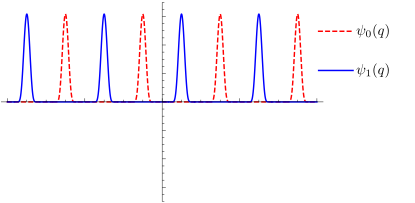
\includegraphics[bb=0bp 90bp 359bp 222bp,clip,width=6cm]{plots/zeroOne}\\
(a) $\left\langle q|\psi_{0}\right\rangle $ (dashed) and $\left\langle q|\psi_{1}\right\rangle $\bigskip{}
\\
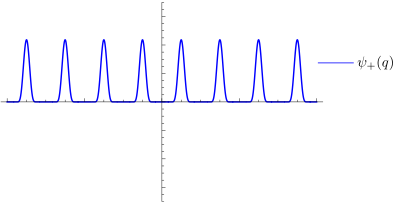
\includegraphics[bb=0bp 90bp 359bp 222bp,clip,width=6cm]{plots/plus}\\
(b) $\left\langle q|\psi_{+}\right\rangle $\bigskip{}
\\
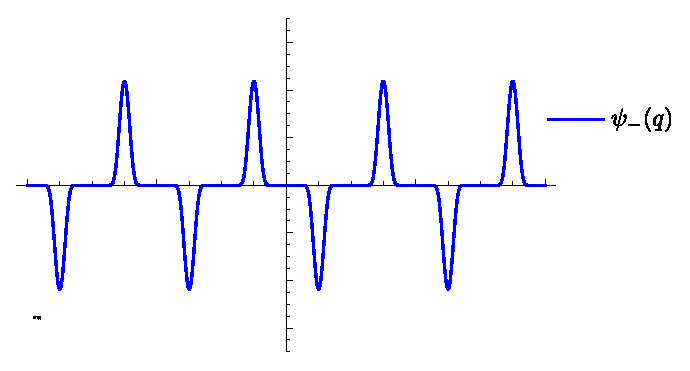
\includegraphics[bb=0bp 20bp 359bp 200bp,clip,width=6cm]{plots/minus}\\
(c) $\left\langle q|\psi_{-}\right\rangle $

\caption{Illustration of $\left|\psi_{\pm}\right\rangle $ and $\left|\psi_{0}\right\rangle ,\,\left|\psi_{1}\right\rangle $
states for $N=8,\, L=1$ unit. The $\left|\psi{}_{0}\right\rangle ,\,\left|\psi_{1}\right\rangle $
states are not normalized.\label{fig:wavefns}}
\end{figure}
Using these states, as illustrated in \figref{wavefns}, we construct the analogues of the $\ket + $ and $\ket - $ states
\[
\left|\psi_{+}\right\rangle \equiv\frac{\left|\psi_{0}\right\rangle +\left|\psi_{1}\right\rangle }{\sqrt{2}},\\
\left|\psi_{-}\right\rangle \equiv\frac{\left|\psi_{0}\right\rangle -\left|\psi_{1}\right\rangle }{\sqrt{2}}
\]
These states were constructed with a partial translational symmetry which is appropriate to the bounded hermitian operator $\hat X$ discussed earlier. It follows that 
\begin{align*}
\bra{\psi_+} \hat X \ket{\psi_+} &= \frac{N-1}{N} \\
\bra{\psi_-} \hat X \ket{\psi_-} &= -\frac{N-1}{N}
\end{align*}
where $N \equiv 2M$ is the number of `slits'.
Before proceeding further, we introduce a unitary operator $\hat U$ to implement different measurement settings. Again, in analogy with the spins\footnote{where a measurement along a vector in the $x-y$ plane for example, maybe made by rotating by an $\phi$, $e^{i\hat{\sigma}_z\phi/2}$ and then measuring $\hat{\sigma}_x$} we define $\hat U$ to be s.t. 
\begin{eqnarray*}
\hat{U}(\phi)\left|\psi_{0}\right\rangle  & = & e^{i\phi/2}\left|\psi_{0}\right\rangle \\
\hat{U}(\phi)\left|\psi_{1}\right\rangle  & = & e^{-i\phi/2}\left|\psi_{1}\right\rangle 
\end{eqnarray*}
This can achieved in principle using alternate glass slabs for photons, to adjust the relative phase as desired, since $\left|\psi_{0}\right\rangle $ and $\left|\psi_{1}\right\rangle $ are spatially separated. Alternatively, we could also define $\hat{U}(\phi)$ in its analytic form. First we claim that $\exists$ an operator $\hat{Z}$ s.t. it satisfies $\hat{Z}\left|\psi_{0}\right\rangle =\left|\psi_{0}\right\rangle $ and $\hat{Z}\left|\psi_{1}\right\rangle =-\left|\psi_{1}\right\rangle $. Before explicitly defining $\hat{Z}$, we observe that given this operator, we can naturally define
\[
\hat{U}(\phi)\equiv e^{i\hat{Z}\phi/2}
\]
It is suggestive from this form that $\hat{Z}$ must play the role of $\hat{\sigma}_z$. We know that $\hat{X}$ is a function of $\hat{p}_{\text{mod}h/L}$. It is thus natural to expect $\hat{Z}$ to be a function of $\hat{q}_{\text{mod}L}$. From it's action, we also note that $\hat{Z}$ must differentiate between spatial wavefunctions $\left\langle q|\varphi\right\rangle $ and $\left\langle q-L|\varphi\right\rangle $. Thus the appropriate operator must be $\hat{q}_{\text{mod}2L}$ and not $\hat{q}_{\text{mod}L}$. This is supported by the fact that $[\hat{p}_{\text{mod}h/L},\hat{q}_{\text{mod}L}]=0$. Now since the action of $\hat{Z}$ must work for arbitrary $\left|\varphi\right\rangle $ and $N$, we define
 \[
\hat{Z}\equiv Z(\hat{q}_{\text{mod}2L})
\]
where $Z$ is some appropriate function, so that $\hat{Z}\left|q\right\rangle =Z(\hat{q}_{\text{mod}2L})\left|q\right\rangle =Z(q_{\text{mod}2L})\left|q\right\rangle $. From the constraints on $\hat{Z}$, we conclude that for consistency, we must define\footnote{$\hat{q}_{\text{mod}2L}$ is well defined, see \subref{c6}}
\[
Z(q)\equiv\begin{cases}
1 & 0<q\le L\\
-1 & L<q\le2L
\end{cases}
\]


\begin{figure}
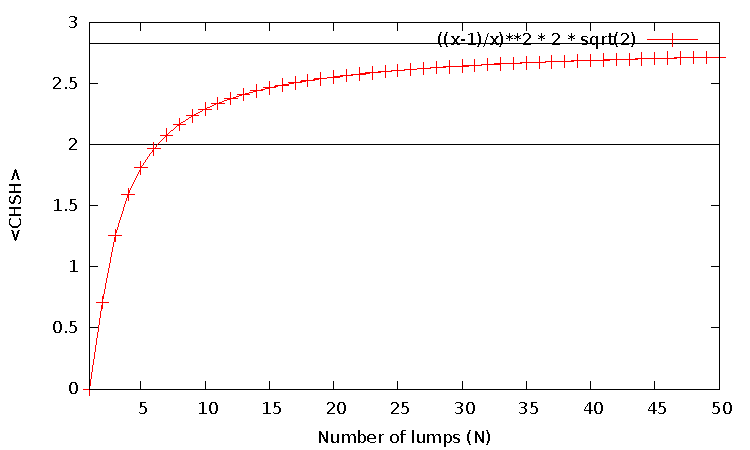
\includegraphics[width=8cm]{plots/CHSH}\caption{Practically, the number of slits, $N$ will be finite. The plot shows
$\braket{ \mathcal {\hat B} } $ as a function of $N$. To get a violation,
we need merely $7$ slits, while with $50$ we are almost at $2\sqrt{2}$.\label{chshViolation}}
\end{figure}


We now describe explicitly, how all these fit with the framework laid out earlier. Consider (a) The first qubit is with Alice and the second with Bob. (b) Alice and Bob apply local unitaries, say $\hat U(\phi)\otimes \mathbb I$ and $\mathbb I \otimes \hat U(\theta)$ respectively and then both measure $\hat X$. (c) Alice can choose between $\phi$ and $\phi'$ and Bob can choose between $\theta$ and $\theta'$.

We claim that the appropriate entangled state which will yield a violation, given the measurement scheme, is
\begin{equation}
\label{entangledState}
\ket{\Psi} \equiv\frac{ \ket{\psi_{+}}_1\ket{\psi_{-}}_2 - \ket{\psi_{-}}_1\ket{\psi_{+}}_2 }{\sqrt{2}}
\end{equation}

Having defined $\Psi$, $\hat A_i$ and $\hat A'_i$, we are now in a position to evaluate $\mean{\mathcal {\hat B}}$. We essentially need terms like $ \mean{ \hat X(\phi) \otimes \hat X(\theta)}$, where $\hat X (\theta) \equiv \hat U^{\dagger}(\theta) \hat X \hat U(\theta)$. It can be shown that (see \subref{c5})
\[
\mean{\hat X(\phi) \otimes \hat X(\theta)} = -\left( \frac{N-1}{N} \right)^2 \cos(\phi-\theta)
\]
Thus for appropriately defiend angles\footnote{One choice is $\theta=0,\theta'=-\pi/2$ and $\phi=3\pi/4,\phi'=3\pi/4 - \pi/2$} we get
 \[
\mean{ \mathcal {\hat B} } =\left(\frac{N-1}{N}\right)^{2}2\sqrt{2}
\] 
The smallest $N$ s.t. $\mean{ \mathcal {\hat B} } >2$, is $N\ge7$; see figure \ref{chshViolation}.


\subsection{Validating phase space behaviour}

%In the past, it has been shown that one can arrive at the violation of the Bell inequality in continuous variable systems. One issue concerning some of these approaches is that the wavefunction used is highly idealized and not normalizable, such as $\left|p\right\rangle $ and $\left|q\right\rangle $ or their countable superposition. Another issue in certain other approaches, is that the wigner functions corresponding to the observables, are unbounded. An example of this is parity. Note that while the Wigner function for a physical state $\rho$ has an upper bound, here we are simply using the prescription to evaluate the same for hermitian operators.

%We care because wigner functions maybe thought of as a specific case of the Wigner-Weyl correspondence, which is a one-one map between classical functions and their corresponding quantum operators. Thus, in a phase-space description of quantum mechanics, it is important to show that it is not necessary to have unboundedness in observables to arrive a violation of the Bell's inequality, and thereby non-locality. 

%In our case, $\left|\Psi\right\rangle $ is manifestly normalized.
To satisfy the assumptions of the framework, we must show that the real function $\mathcal W_{\hat X(\phi)}\le 1$. To that end, we note that

%\begin{widetext}

%\end{widetext}

\begin{eqnarray*}
\mathcal W_{\hat X (\phi)}(q,p) & = & \frac{1}{2}\int dq'e^{ipq'/\hbar} \bra{q-\frac{q'}{2}}\bigg( e^{-i\hat Z\phi/2}\\
 &  & e^{i\hat{p}\frac{L}{\hbar}}e^{i\hat Z\phi/2} + \text{h.c.} \bigg) \ket{q+\frac{q'}{2}}\\
 & = & \frac{1}{2}\left( e^{-iZ_{-}(q)\phi/2}e^{ip\frac{L}{\hbar}}e^{iZ_{+}(q)\phi/2}\right) + \text{h.c.}\\
 & = & \cos(pL/\hbar \pm Z_{\pm}(q)\phi) \le 1
\end{eqnarray*}
where $Z_{\pm}(q) \equiv Z[(q\pm\frac{L}{2})\text{mod}2L]$ and we used the fact that $Z(x)=-Z(x+L)$ (omitting the $\text{mod}2L$). %Manifestly then, $\left| \mathcal W_{\hat A_i}\right|, \left| \mathcal W_{\hat A'_i}\right|  \le 1$ as was claimed.


\subsection{Commutations and Violation}

In the Bell test done with spins, the source of violation hinges on the non-commutativity of the Pauli matrices. It is known that $C^{2}=4\mathbb{I}+[a_{1},a_{2}]\otimes[b_{1},b_{2}]$, when $a_{i},b_{i}\in\{-1,1\}$. To obtain a violation in general (where the first term maybe less than $4\mathbb{I}$), it is therefore necessary that the commutations don't vanish. This is indeed true in our case. Explicitly, we must have $[\hat X(\phi),\hat X (\phi')]\neq0$. To arrive at the desired expression we first evaluate some simpler
commutation and anti-commutation relations explicitly. Let's start with $[\hat{Z},e^{i\hat{p}L/\hbar}]=\hat{Z}e^{i\hat{p}L/\hbar}-e^{i\hat{p}L/\hbar}\hat{Z}$.
To evaluate it, we multiply the second term with $\int dx\left|x\right\rangle \left\langle x\right|$ and obtain $\hat Ze^{i\hat{p}L/\hbar}+\hat Ze^{i\hat{p}L/\hbar}$ where we've
used $Z(\hat{x}_{\text{mod}2L})=-Z(\left(\hat{x}\pm L\right)_{\text{mod}2L})$ and $e^{i\hat{p}L/\hbar}\left|x\right\rangle =\left|x-L\right\rangle $.
Thus we have 
\[
[\hat{Z},\hat{X}]=2\hat{Z}\hat{X}=-2i\hat{Y}
\]
where $\hat{Y}=i\hat{Z}\hat{X}$. Here $i$ was introduced to ensure $\hat{Y}^{\dagger}=\hat{Y}$, since $\hat{X}^{\dagger}=\hat{X}$ and $\hat{Z}^{\dagger}=\hat{Z}$. Similarly it follows that $\{\hat{Z},\hat{X}\}=0$. From the definition of $Y$ and the anti-commutation, $\{\hat{Y},\hat{X}\}=0$ and $\{\hat{Y},\hat{Z}\}=0$ also follow trivially. We may point out that while $\hat{Z}^{2}=1$, it is not a sum of a 2 state projector and $\hat{X}^{2}\neq1$ in general. This manifests in the following relations 
\begin{eqnarray*}
[\hat{X},\hat{Y}] & = & -2i\hat{Z}\hat{X}^{2}=-2i\hat{X}^{2}\hat{Z}\\{}
[\hat{Y},\hat{Z}] & = & -2i\hat{X}
\end{eqnarray*}
Further, note that $e^{-i\hat{Z}\phi/2}\hat{X}e^{i\hat{Z}\phi/2}=\hat{X}e^{i\hat{Z}\phi}$ and that $e^{i\hat{Z}\phi}=\cos\phi+i\hat{Z}\sin\phi$. 
With all these, it is easy to show that 
\begin{eqnarray*}
[\hat{U}^{\dagger}(\frac{\phi}{2})\hat{X}\hat{U}(\frac{\phi}{2}),\hat{U}^{\dagger}(\frac{\phi'}{2})\hat{X}\hat{U}(\frac{\phi'}{2})] & =\\
\left(\cos\phi\sin\phi'-\sin\phi\cos\phi'\right)\hat{Z}\hat{X}^{2} & \neq & 0
\end{eqnarray*}
as was necessary. Ofcourse this is not sufficient, however we have shown explicitly the violation. This evaluation was meant to illuminate that the source of violation essentially hinges on $[\hat{x},\hat{p}]=i\hbar$. It is apparent that the complete pauli algebra is unnecessary for
showing a violation. 


\subsection{Advantage of asymmetry in $\hat{X}$ and $\hat{Z}$}

Considering the operator (non-hermitian for simplicity) $\hat{X}=e^{i\hat{p}L/\hbar}$, defining $\hat{Z}=e^{i\hat{q}2\pi/2L}$ is more natural. They also follow the desired anti-commutation $\{\hat{X},\hat{Z}\}=0$ and we could define $\hat{Y}=\hat{iZ}\hat{X}$ to get a more natural generalization. The question is why did $\hat{Z}=Z(\hat{q}_{\text{mod}2L})$ appear in the analysis. The cause of this asymmetry hinges on the preferential treatment of position space. We could have constructed states of the form $\left|\psi_{0}\right\rangle =\sum_{n}\left|q+nd\right\rangle $ and used the natural definition of $\hat{Z}$ to obtain the violation. The issue is that this forces us to choose a countable superposition of position eigenkets as our desired state. Such a state is strictly not even in the Hilbert space. In the scheme proposed, this issue is resolved by $Z(\hat{q}_{\text{mod}2L})$ which causes a larger set of physically realizable states to become admissible.
Thus while our construction is motivated by the spin formalism, it is not just a relabelling of states and operators achieved by a severe restriction of the Hilbert space. 


\section{Physical Implementation}

We show that this scheme can be implemented rather easily using photons. We harness the two degrees of freedom of a photon, it's polarization and it's position to construct the required state. With a slightly modified setup, it is possible to do the same with spin and position
for matter waves (see \subref{c7}). The overall setup (see \figref{scheme}) is such that we need only consider the quantum mechanical description along the $x$-axis.


\subsection{Creation of the entangled state}

The desired entangled state is $\ket{\Psi}$, as stated in equation \ref{entangledState}. 
We start with noting the triviality of constructing a 
\[
\left|\psi_{+}\right\rangle =\frac{1}{\sqrt{N}}\sum_{n\in I_{N}}\left|\varphi_{n}\right\rangle 
\]
 state. One simply needs a source and a grating, viz. a screen with $N$ slits of width $a\ll L$, separated by a distance $L$ (centre to centre). The 
\[
\left|\psi_{-}\right\rangle =\frac{1}{\sqrt{N}}\sum_{n\in I_{N}}\left(-1\right)^{n+1}\left|\varphi_{n}\right\rangle 
\]
 state can be similarly constructed by using glass slabs at alternate slits, such that the phase introduced is $\pi\,\implies\, e^{i\pi}=-1$. In \figref{scheme}, if you consider only one particle, and disregard
everything after the grating, then the setup is expected to produce a $\left|\psi_{+}\right\rangle $ state, just after the grating. To produce the desired entangled state, we start with two entangled photons, such that their polarization state can be expressed as $\ket{\chi} \equiv \frac{ \ket{H}_1\ket{V}_2 -\ket{V}_1\ket{H}_2 }{\sqrt{2}}$. Their spatial description (along $x$-axis) is initially assumed to be $\ket{\gamma}_1 \ket{\gamma}_2$.

The state $\left|\gamma\right\rangle $ maybe considered to be a Gaussian with $\sigma\gg2NL$ so that after the grating, the spatial state can be written as 
\[
\frac{ \ket{H}_1\ket{V}_2 -\ket{V}_1\ket{H}_2 }{\sqrt{2}} \ket{\psi_+}_1\ket{\psi_+}_2
\]
To produce a $\left|\psi_{-}\right\rangle $ state, we already know we needed alternate glass slabs. If we had glass slabs, whose refractive index (given some orientation) was say $\eta_{H}=1$ for a horizontally polarized beam and $\eta_{V}=\eta\neq1$ for vertical polarization, then we could harness the entangled polarization state to create the required spatially entangled state. Birefringent crystals have such polarization dependent refractive indices. Assume that alternating birefringent crystals have been placed after both the gratings %as shown in \figref{scheme} (in the diagram, they're not alternating for reasons to follow). 
These have widths such that the resultant phase it introduces is $\pi$ and the state is 

\[
\frac{\ket{H}_1\ket{V}_2\ket{\psi_+}_1\ket{\psi_-}_2 - \ket{V}_1\ket{H}_2\ket{\psi_-}_1\ket{\psi_+}_2}{\sqrt 2} 
\]
At this stage, if we were to trace out the polarization state, we'd
end up with a mixed state. That is useless for our test. Ignoring
the glass slabs at the moment in \figref{scheme}, we observe the
action of the polarisers on the state. After the $45^{\circ}$ polariser,
the state becomes (see \subref{c8}) 
\[
\ket{\chi_{45}}\ket{\Psi} = \ket{\nearrow}_1\ket{\nearrow}_2 \frac{\ket{\psi_+}_1\ket{\psi_-}_2 - \ket{\psi_-}_1\ket{\psi_+}_2}{\sqrt 2}
\]
where $\left|\nearrow\right\rangle \equiv\left(\left|H\right\rangle +\left|V\right\rangle \right)/\sqrt{2}$.
Now if we trace out the polarization state, we'd be left with the target entangled state. As a remark, it maybe be stated that although to arrive at this result we assumed that $\eta_{H}=1$, which is unreasonable physically, we can compensate for $\eta_{H}\neq1$ by putting appropriate glass slabs at the alternate empty slits, to produce zero relative phase when the polarization is horizontal.

\begin{figure*}
\resizebox{15cm}{!}{\begin{picture}(0,0)%
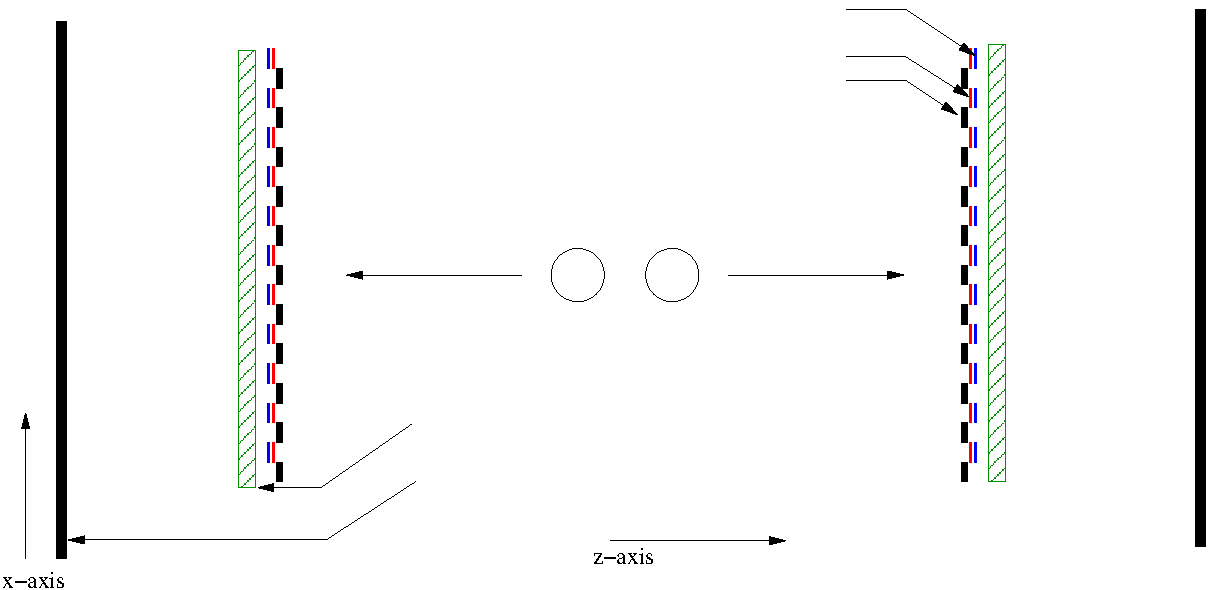
\includegraphics{/afs/tp.nt.uni-siegen.de/user/arora/Documents/projectSiegen/firstDraft/diagrams/scheme}%
\end{picture}%
\setlength{\unitlength}{4144sp}%
%
\begingroup\makeatletter\ifx\SetFigFont\undefined%
\gdef\SetFigFont#1#2#3#4#5{%
  \reset@font\fontsize{#1}{#2pt}%
  \fontfamily{#3}\fontseries{#4}\fontshape{#5}%
  \selectfont}%
\fi\endgroup%
\begin{picture}(9215,4490)(751,-4486)
\put(5431,-421){\makebox(0,0)[lb]{\smash{{\SetFigFont{12}{14.4}{\rmdefault}{\mddefault}{\updefault}{\color[rgb]{1,0,0}Birefringent Crystals}%
}}}}
\put(6121,-151){\makebox(0,0)[lb]{\smash{{\SetFigFont{12}{14.4}{\rmdefault}{\mddefault}{\updefault}{\color[rgb]{0,0,1}Glass slabs}%
}}}}
\put(6451,-691){\makebox(0,0)[lb]{\smash{{\SetFigFont{12}{14.4}{\rmdefault}{\mddefault}{\updefault}{\color[rgb]{0,0,0}Grating}%
}}}}
\put(4951,-1726){\makebox(0,0)[lb]{\smash{{\SetFigFont{12}{14.4}{\rmdefault}{\mddefault}{\updefault}{\color[rgb]{0,0,0}$\ket{\chi} = (\ket{HV} - \ket{VH})/\sqrt 2$}%
}}}}
\put(3916,-3616){\makebox(0,0)[lb]{\smash{{\SetFigFont{12}{14.4}{\rmdefault}{\mddefault}{\updefault}{\color[rgb]{0,0,0}Screen}%
}}}}
\put(3916,-3256){\makebox(0,0)[lb]{\smash{{\SetFigFont{12}{14.4}{\rmdefault}{\mddefault}{\updefault}{\color[rgb]{0,0,0}$45^o$ polarizer}%
}}}}
\end{picture}%
}

\caption{Scheme for creating the state\label{fig:scheme}}
\end{figure*}



\subsection{Measurement Settings}

In our scheme, Alice and Bob can choose between $\phi,\phi'$ and $\theta,\theta'$ respectively. To implement this, we recall that the action of $\hat{U}(\theta)$, is to introduce a phase difference between the $\left|\psi_{0}\right\rangle $ and $\left|\psi_{1}\right\rangle $ states. By construction, $\left|\psi_{0}\right\rangle $ and $\left|\psi_{1}\right\rangle $ are spatially disjoint; thus the operation of $\hat{U}(\theta)$ can be implemented by simply placing alternating glass slabs at the slits, with widths such that $\left|\psi_{0}\right\rangle \to e^{i\theta/2}\left|\psi_{0}\right\rangle $ and $\left|\psi_{1}\right\rangle \to e^{-i\theta/2}\left|\psi_{1}\right\rangle $. The same operation maybe done for $\hat{U}(\phi)$ for the second particle. In the overall scheme, %as shown in \figref{scheme}, 
this is can be done by placing glass slabs right after the birefringent crystals. The state after application of the unitaries is given by $\left|\Psi_{f}\right\rangle $, where $f$ is used to index which of the four possible measurement settings was used. 

\subsection{Effective Practical Setup}

Placing glass slabs may not be suitable for fine gratings. Thus practically we can implement the same scheme using the setup shown in figure []. First we note that only relative phases between $\ket{\psi_0}$ and $\ket{\psi_1}$ are essential. The first large slab is a Birefringent crystal ($\eta_H,\eta_V$) while the adjacent slab is plain glass ($\eta$). We generate longitudenal standing pressure waves so that the effective thickness at alternate grating sites are given by $d_0,d_1$ and $t_0,t_1$ for the crystal and slab respectively. The phase difference between a horiztonal $\ket{\psi_0}$ and $\ket{\psi_1}$ will be given by $\eta_H(d_0 - d_1)\equiv \theta_A$. For the vertical component, it'll be $\eta_V(d_0-d_1)$. If we impose $\eta_V(d_0-d_1)=\pi+\theta_A$, then we would've created\footnote{upto an overall phase} the state $e^{i\hat Z \theta_A}\frac{\ket{\psi_+} + \ket{\psi_-}}{\sqrt{2}}$ for an incident $\frac{\ket{H}+\ket{V}}{\sqrt{2}}$ polarization state. $d_0$ and $d_1$ will be constrained by some relation depending on physical properties of the crystal; it'll also depend on the amplitude of the longitudenal wave. From this and the imposed constrain, $d_0,d_1$ can be determined. However, we haven't the freedom to change $\theta_A$. To remedy this, we use the glass slab. It will introduce a phase $\eta(t_0-t_1)\equiv \theta_B$. Here, again $t_0,t_1$, may satisfy some constraint, but will depend on the amplitude which is adjustable. Thus effectively, by changing this amplitude, we can set the relative phase $\theta=\theta_A+\theta_B$ arbitrarily. Effectively therefore, this scheme allows for both creation of the entangled state and changing the measurement settings in a practical way.


\subsection{Measurement}

The scheme requires us to evaluate the expectation value of $\hat{X}\otimes\hat{X}$
(after the measurement settings have been applied by the appropriate
unitaries). If from the experiment, we can obtain the probability
$\left|\left\langle p{}_{A},p{}_{B}|\Psi_{f}\right\rangle \right|^{2}$,
then evaluating $\braket{ \hat{X}\otimes\hat{X} } =\left\langle \cos(\hat{p}L/\hbar)\otimes\cos(\hat{p}L/\hbar)\right\rangle $
simply amounts to $\int dp{}_{A}dp{}_{B}\cos(p{}_{A}L/\hbar)\cos(p{}_{B}L/\hbar)\left|\left\langle p{}_{A},p{}_{B}|\Psi_{f}\right\rangle \right|^{2}$. 

Therefore it is sufficient to explain how to obtain the joint momentum
probability distribution from the experiment, for a given measurement
setting. We start with stating the result that in the far-field approximation,
\begin{equation}
\label{eqn:measure}
\left| \braket{q_A,q_B | \Psi_{f\text{ screen}}} \right|^2 \propto \left| \braket{p_A=\frac{p_zq_A}{D},p_B=\frac{p_zq_B}{D}|\Psi_f} \right|^2
\end{equation}
 where $\left|\Psi{}_{f\,\text{screen}}\right\rangle $ is the state of the system at the screen, $D$ is the distance between the gratings
and the screens and $p_{z}$ is the $z$ component of momentum of the particle. For a photon, $p_{z}=h/\lambda$ while for an electron, $p_{z}=m_{e}D/T$, where $T$ is the time taken to arrive at the screen from the grating. The idea is simply that the momentum distribution at the grating can be recovered by observing the spatial distribution at a screen, sufficiently far away.
In an experiment then, there are two possibilities. \\
(a) Given $f$, Alice and Bob both note the position at which they obtain their particle. After repeating the experiment sufficiently many times, they share their list to create a sequence $\{(q{}_{A}^{(i)},q_{B}^{(i)})\}$. From this sequence, they create a 2D histogram, by simply counting how many time they got $(q'_{A},q'_{B})$ to lie inside a given cell. The normalized result is essentially $\left|\left\langle q{}_{A},q{}_{B}|\Psi{}_{f\,\text{screen}}\right\rangle \right|^{2}$
from which $\braket{ \hat{X}\otimes\hat{X} }$ can be computed as discussed. $f$ is changed to evaluate all the 4 terms to finally obtain $\braket{ \hat{\mathcal{B}} }$ experimentally. For details, see section \ref{sub:c9}.
\\
(b) The other simpler, equivalent and direct possibility is that Alice and Bob both obtain the position, $(q_{A}^{(i)},q_{B}^{(i)})$ for the $i$th repetition and evaluate $\cos(p_{A}^{(i)}L/\hbar)$ and $\cos(p_{B}^{(i)}L/\hbar)$. After sufficient iterations (for all values of $f$), they exchange their observations to simply evaluate
the average, viz. 
\[
\frac{\sum_{i}\cos(p_{A}^{(i)}L/\hbar)\cos(p_{B}^{(i)}L/\hbar)}{\sum_{i}}=\braket{ \hat{\mathcal{B}} }
\]



\section{Conclusion}

come up with a scheme for local realism test which verify or disprove quantum mechanics predictions  with most ``classical-like'' measurements and operations.

We have shown how to realize a Bell test in continuous variables position
and momentum using specifically chosen and physically realizable states.
In addition it has been demonstrated that the exact pauli commutation
relations aren't necessary to capture the essence of non-locality;
infact by relaxing the similarity, the set of states that show a violation
is made considerably larger.


\section{Appendix}


\subsubsection*{Illustration (I)}

This is trival if one uses the Bloch sphere picture. Instead of measuring
along an arbitrary axis, we rotate the Bloch sphere appropriately,
and then measure $x$. To illustrate this, consider
\begin{lyxlist}{a}
\item [{Questn:}] $\exists\,\text{a}\,\hat{U},\, s.t.\,\text{if}\,\left|\chi\right\rangle \to\left|\chi'\right\rangle =\hat{U}\left|\chi\right\rangle \,\mbox{\text{then}\,}\left\langle \chi\left|\hat{x}\right|\chi\right\rangle =\left\langle \chi'\left|\hat{y}\right|\chi'\right\rangle $?
\\
Explicitly, we have 
\begin{eqnarray*}
\hat{y} & = & \hat{U}^{\dagger}\hat{x}\hat{U}=e^{-i\hat{z}\theta/2}\hat{x}e^{i\hat{z}\theta/2}\\
 & = & \hat{x}e^{i\hat{z}\theta}=\left[\begin{array}{cc}
0 & 1\\
1 & 0
\end{array}\right]\left[\begin{array}{cc}
e^{i\theta} & 0\\
0 & e^{-i\theta}
\end{array}\right]\\
 & = & \left[\begin{array}{cc}
0 & -i\\
i & 0
\end{array}\right]
\end{eqnarray*}
for $\theta=\pi/2$ as one would guess geometrically. 
\end{lyxlist}

\subsection*{Claims}


\subsubsection{If $\left|\psi\right\rangle \equiv\frac{\left|+-\right\rangle -\left|-+\right\rangle }{\sqrt{2}}$,
then$\left|\psi\right\rangle =\frac{\left|10\right\rangle -\left|01\right\rangle }{\sqrt{2}}$\label{sub:c1}}


\subsubsection{$\left\langle x\otimes x\right\rangle =-1$, for $\left|\psi\right\rangle $
in Claim(1)\label{sub:c2}}


\subsubsection{$\left\langle e^{-iz\theta/2}xe^{iz\theta/2}\otimes e^{-iz\phi/2}xe^{iz\phi/2}\right\rangle =-\cos(\phi-\theta)$\label{sub:c3}}

Proof: 
\begin{eqnarray*}
\text{LHS} & = & \left\langle xe^{-iz\theta}\otimes xe^{iz\phi}\right\rangle \\
 & = & \left[\frac{\left\langle 10\right|-\left\langle 01\right|}{\sqrt{2}}\right]\left[xe^{iz\theta}\otimes xe^{iz\phi}\right]\left[\frac{\left|10\right\rangle -\left|01\right\rangle }{\sqrt{2}}\right]\\
 & = & \left\langle \psi\right|x\otimes x\\
 &  & \Bigg[\frac{e^{i\left(\phi-\theta\right)}\left(\frac{\left|+\right\rangle -\left|-\right\rangle }{\sqrt{2}}\right)\left(\frac{\left|+\right\rangle +\left|-\right\rangle }{\sqrt{2}}\right)}{\sqrt{2}}\\
 &  & -\frac{e^{-i\left(\phi-\theta\right)}\left(\frac{\left|+\right\rangle +\left|-\right\rangle }{\sqrt{2}}\right)\left(\frac{\left|+\right\rangle -\left|-\right\rangle }{\sqrt{2}}\right)}{\sqrt{2}}\Bigg]
\end{eqnarray*}
We define, $\delta\equiv\phi-\theta$ and using \subref{c1}, it follows
that only terms like $\left|+-\right\rangle $ or $\left|-+\right\rangle $;
so
\begin{eqnarray*}
\text{LHS} & = & \left\langle \psi\right|x\otimes x\\
 &  & \left[\frac{e^{i\delta}\left(\frac{\left|+-\right\rangle -\left|-+\right\rangle }{2}\right)-e^{-i\delta}\left(\frac{-\left|+-\right\rangle +\left|-+\right\rangle }{2}\right)}{\sqrt{2}}\right]\\
 & = & \left\langle \psi\right|x\otimes x\left[\frac{e^{i\delta}\left(\frac{\left|\psi\right\rangle }{\sqrt{2}}\right)+e^{-i\delta}\left(\frac{\left|\psi\right\rangle }{\sqrt{2}}\right)}{\sqrt{2}}\right]\\
 & =- & \frac{e^{i\delta}+e^{-i\delta}}{2}\\
 & =- & \cos(\phi-\theta)
\end{eqnarray*}
where we've used \subref{c2}.


\subsubsection{Without taking the large $N$ limit\label{sub:c4}}

$\left\langle \psi_{+}\left|\hat{X}\right|\psi_{+}\right\rangle =\frac{N-1}{N}$,
$\left\langle \psi_{-}\left|\hat{X}\right|\psi_{-}\right\rangle =-\frac{N-1}{N}$\\
$\left\langle \psi_{0}\left|\hat{X}\right|\psi_{0}\right\rangle =0$,
$\left\langle \psi_{1}\left|\hat{X}\right|\psi_{1}\right\rangle =0$\\
$\left\langle \psi_{1}\left|\hat{X}\right|\psi_{0}\right\rangle =\frac{\frac{N-1}{N}+\frac{N}{N}}{2}=\frac{2N-1}{2N}=\left\langle \psi_{0}\left|\hat{X}\right|\psi_{1}\right\rangle $\\
$\left\langle \psi_{-}\left|\hat{X}\right|\psi_{+}\right\rangle =\frac{-\left\langle \psi_{1}\left|\hat{X}\right|\psi_{0}\right\rangle +\left\langle \psi_{0}\left|\hat{X}\right|\psi_{1}\right\rangle }{2}=0=\left\langle \psi_{+}\left|\hat{X}\right|\psi_{-}\right\rangle $\\
\begin{eqnarray*}
\left\langle \Psi\left|\hat{X}\otimes\hat{X}\right|\Psi\right\rangle  & = & \frac{1}{2}\bigg(\left\langle \psi_{-}\left|\hat{X}\right|\psi_{-}\right\rangle \left\langle \psi_{+}\left|\hat{X}\right|\psi_{+}\right\rangle +\\
 &  & \left\langle \psi_{+}\left|\hat{X}\right|\psi_{+}\right\rangle \left\langle \psi_{-}\left|\hat{X}\right|\psi_{-}\right\rangle \bigg)\\
 & = & -\left(\frac{N-1}{N}\right)^{2}
\end{eqnarray*}



\subsubsection{For arbitrary $\theta_{i}$ and $\phi_{i}$ $\left\langle \hat{U}^{\dagger}(\phi_{i})\hat{X}\hat{U}(\phi_{i})\otimes\hat{U}^{\dagger}(\theta_{i})\hat{X}\hat{U}(\theta_{i})\right\rangle =-\left(\frac{N-1}{N}\right)^{2}\cos(\phi_{i}-\theta_{i})$\label{sub:c5}}

Proof: We start with defining $\phi\equiv\phi_{i}$ , $\theta\equiv\theta_{i}$,
$\delta\equiv\phi-\theta$, $\delta'\equiv\delta/2$. Next, we note
that $\text{LHS}=\left\langle \Psi'\left|\hat{X}\otimes\hat{X}\right|\Psi'\right\rangle $
where $\left|\Psi'\right\rangle =\hat{U}(\phi_{i})\otimes\hat{U}(\theta_{i})\left|\Psi\right\rangle $.
\begin{eqnarray*}
\left|\Psi'\right\rangle  & = & \frac{e^{i\delta'}}{\sqrt{2}}\left(\frac{\left|\psi_{+}\right\rangle -\left|\psi_{-}\right\rangle }{\sqrt{2}}\right)\left(\frac{\left|\psi_{+}\right\rangle +\left|\psi_{-}\right\rangle }{\sqrt{2}}\right)\\
 &  & -\frac{e^{-i\delta'}}{\sqrt{2}}\left(\frac{\left|\psi_{+}\right\rangle +\left|\psi_{-}\right\rangle }{\sqrt{2}}\right)\left(\frac{\left|\psi_{+}\right\rangle -\left|\psi_{-}\right\rangle }{\sqrt{2}}\right)\\
 & = & \frac{e^{i\delta'}}{2\sqrt{2}}\left(\left|\psi_{+}\psi_{+}\right\rangle +\left|\psi_{+}\psi_{-}\right\rangle -\left|\psi_{-}\psi_{+}\right\rangle -\left|\psi_{-}\psi_{-}\right\rangle \right)\\
 &  & -\frac{e^{-i\delta'}}{2\sqrt{2}}\left(\left|\psi_{+}\psi_{+}\right\rangle -\left|\psi_{+}\psi_{-}\right\rangle +\left|\psi_{-}\psi_{+}\right\rangle -\left|\psi_{-}\psi_{-}\right\rangle \right)\\
 & = & \frac{e^{i\delta'}-e^{-i\delta'}}{2\sqrt{2}}\left|\psi_{+}\psi_{+}\right\rangle +\frac{e^{i\delta'}+e^{-i\delta'}}{2\sqrt{2}}\left|\psi_{+}\psi_{-}\right\rangle \\
 &  & -\left(\frac{e^{i\delta'}+e^{-i\delta'}}{2\sqrt{2}}\right)\left|\psi_{-}\psi_{+}\right\rangle -\left(\frac{e^{i\delta'}-e^{-i\delta'}}{2\sqrt{2}}\right)\left|\psi_{-}\psi_{-}\right\rangle 
\end{eqnarray*}
Now using \subref{c4}, we have
\begin{eqnarray*}
\text{LHS} & = & \left\langle \Psi'\left|\hat{X}\otimes\hat{X}\right|\Psi'\right\rangle \\
 & = & \frac{1}{2}\left(\frac{N-1}{N}\right)^{2}\Bigg[\left|\frac{e^{i\delta'}-e^{-i\delta'}}{2}\right|^{2}\\
 &  & -\left|\frac{e^{i\delta'}+e^{-i\delta'}}{2}\right|^{2}-\left|\frac{e^{i\delta'}+e^{-i\delta'}}{2}\right|^{2}\\
 &  & +\left|\frac{e^{i\delta'}-e^{-i\delta'}}{2}\right|^{2}\Bigg]\\
 & = & -\left(\frac{N-1}{N}\right)^{2}\frac{1}{2}\left[2\left(\cos^{2}\delta/2-\sin^{2}\delta/2\right)\right]\\
 & = & -\left(\frac{N-1}{N}\right)^{2}\cos\left(\delta\right)
\end{eqnarray*}



\subsubsection{Action of $\hat{x}_{\text{mod}2L}$ can be defined explicitly\label{sub:c6}}

Proof: $\hat{x}_{\text{mod}2L}\equiv\int dxx{}_{mod2L}\left|x\right\rangle \left\langle x\right|$.
To arrive at this more carefully, consider the operator $e^{i\hat{x}\frac{2\pi}{2L}}$.
Note that $e^{i\hat{x}\frac{2\pi}{2L}}\left|x\right\rangle =e^{ix\frac{2\pi}{2L}}\left|x\right\rangle =e^{ix{}_{mod2L}\frac{2\pi}{2L}}\left|x\right\rangle $.
Thus, $\hat{x}_{\text{mod}2L}\left|x\right\rangle =x{}_{mod2L}\left|x\right\rangle $,
consequently on the most general state $\left|f\right\rangle \equiv\int dxf_{x}\left|x\right\rangle $
then, we'd have $\hat{x}_{\text{mod}2L}\left|f\right\rangle =\int dxf_{x}x{}_{mod2L}\left|x\right\rangle $. 

Remark: One needn't necessarily consider eigenstates of $\hat{x}$
to define the action. Eigenstates of $e^{i\hat{x}\frac{2\pi}{2L}}$
maybe considered instead; they can be expressed as (a) $\left|\varphi\right\rangle ,\, s.t.\,\left\langle p+\frac{h}{2L}|\varphi\right\rangle =\left\langle p|\varphi\right\rangle ,\,\forall\, p\in\mathbb{R}$
or (b) $\left|\bar{x}\right\rangle \propto\sum_{n\in\mathbb{Z}}\left|\bar{x}+n2L\right\rangle $.
Using the second expression, we have $e^{i\hat{x}\frac{2\pi}{2L}}\left|\bar{x}\right\rangle =e^{i\bar{x}\frac{2\pi}{2L}}\left|\bar{x}\right\rangle $.
Thus on a more general state, $\left|c\right\rangle \equiv\int_{0}^{2L}d\bar{x}c_{\bar{x}}\left|\bar{x}\right\rangle $,
we have $\hat{x}_{\text{mod}2L}\left|c\right\rangle =\int_{0}^{2L}d\bar{x}c_{\bar{x}}\bar{x}\left|\bar{x}\right\rangle $. 

\smallskip{}



\subsubsection{Physical implementation with electrons is also possible\label{sub:c7}}

If we can show that the basic components used to describe the photon
setup can be translated to the electron setup, then in principle we
are through. (a) Glass slab: The equivalent is the electric AB effect.
We need to simply put a capacitor after the slit and the two components
will pick up a phase difference. (b) Polariser: The Stern Gerlach
setup is the classic analogue. We simply block the orthogonal component.
(c) Birefringent crystal: This is slightly tricky. It can be modelled
by using a combination of gradient of magnetic field (as in Stern
Gerlach) and a capacitor. We start with an equivalent superposition
of spin states, $\frac{\left|\uparrow\downarrow\right\rangle -\left|\downarrow\uparrow\right\rangle }{\sqrt{2}}\left|\psi_{+}\psi_{+}\right\rangle $.
To construct the spin dependent $\left|\psi_{-}\right\rangle $ state,
we use the magnetic field gradient to spatially separate the $\left|\uparrow\right\rangle $
and $\left|\downarrow\right\rangle $ states. We place capacitors
as described at the spatial position corresponding to $\left|\downarrow\right\rangle $
say. Thereafter, we remove the magnetic field gradient and allow the
beams to meet again. This will effectively act as a Birefringent crystal,
since the phase difference is spin dependent.


\subsubsection{Action of a polariser\label{sub:c8}}

If we define $\left|\nearrow\right\rangle \equiv\frac{\left|H\right\rangle +\left|V\right\rangle }{\sqrt{2}},$
$\left|\nwarrow\right\rangle \equiv-\frac{\left|H\right\rangle -\left|V\right\rangle }{\sqrt{2}}$
and the $45^{\circ}$ projector as $\left|\nearrow\right\rangle \left\langle \nearrow\right|$,
then both $\left|H\right\rangle \to\left|\nearrow\right\rangle $ and $\left|V\right\rangle \to\left|\nearrow\right\rangle$
where ofcourse with a probability $1/2$, the photon will be lost.


\subsubsection{More on measurement\label{sub:c9}}
It is essential to know what ballpark resolution is required for detecting the violation from the screen. The histogram discussed in sec [], will be given by $\left| \braket{p_1,p_2|\Psi_f} \right| ^2$. If our measurement can faithfully resolve this, it follows from our previous discussions that a violation will be obtained. This expression may be explicitly evaluated from
\[
\braket{p_1, p_2 | \Psi_f}=\frac{1}{\sqrt 2} \tilde{\varphi}(p_1) \tilde{\varphi}(p_2) F_f(p_1,p_2)
\]
with
\begin{align*}
F_f(p_1,p_2)&=\sum_{(n,m)\in I_N \otimes I_N} e^{i(np_1 + mp_2)L/\hbar} \\
& \left[ -\cos(\delta') [(-)^m - (-)^n] + i \sin(\delta') [1 + (-)^{n+m}] \right]
\end{align*}

where $\tilde{\varphi}(p) \equiv \braket{p|\varphi}$ and $\delta' = (\phi - \theta)/2$. Here the information about $\delta'$ is contained in $f$, and $N$ is known from $\ket{\Psi}$. Since the wavefunction $\varphi(q)$ was assumed sharp with respect to $L$, $\ab{ \tilde \phi(p)}$ will only correspond to a broad envelope, over the range $(-Nh/2L,Nh/2L)$. Thus the main feature of $\ab{\tilde \Psi_f}^2$ will be given by $\ab{F_f}^2$ as shown in figure \ref{fig:psiTilde}. Graphically it is clear that a resolution of about $\frac{1}{10}p_{\text{typ}}=\frac{1}{10}\frac{h}{L}$ should be sufficient to capture the relevant features. On the screen, this translates to a typical length, $q_{\text{typ}}=\lambda D /L$ which follows from equation \ref{eqn:measure} and $p_z=h/\lambda$ for a photon. This is reminiscent of typical diffraction experiments and is readily measurable.

\begin{figure}
  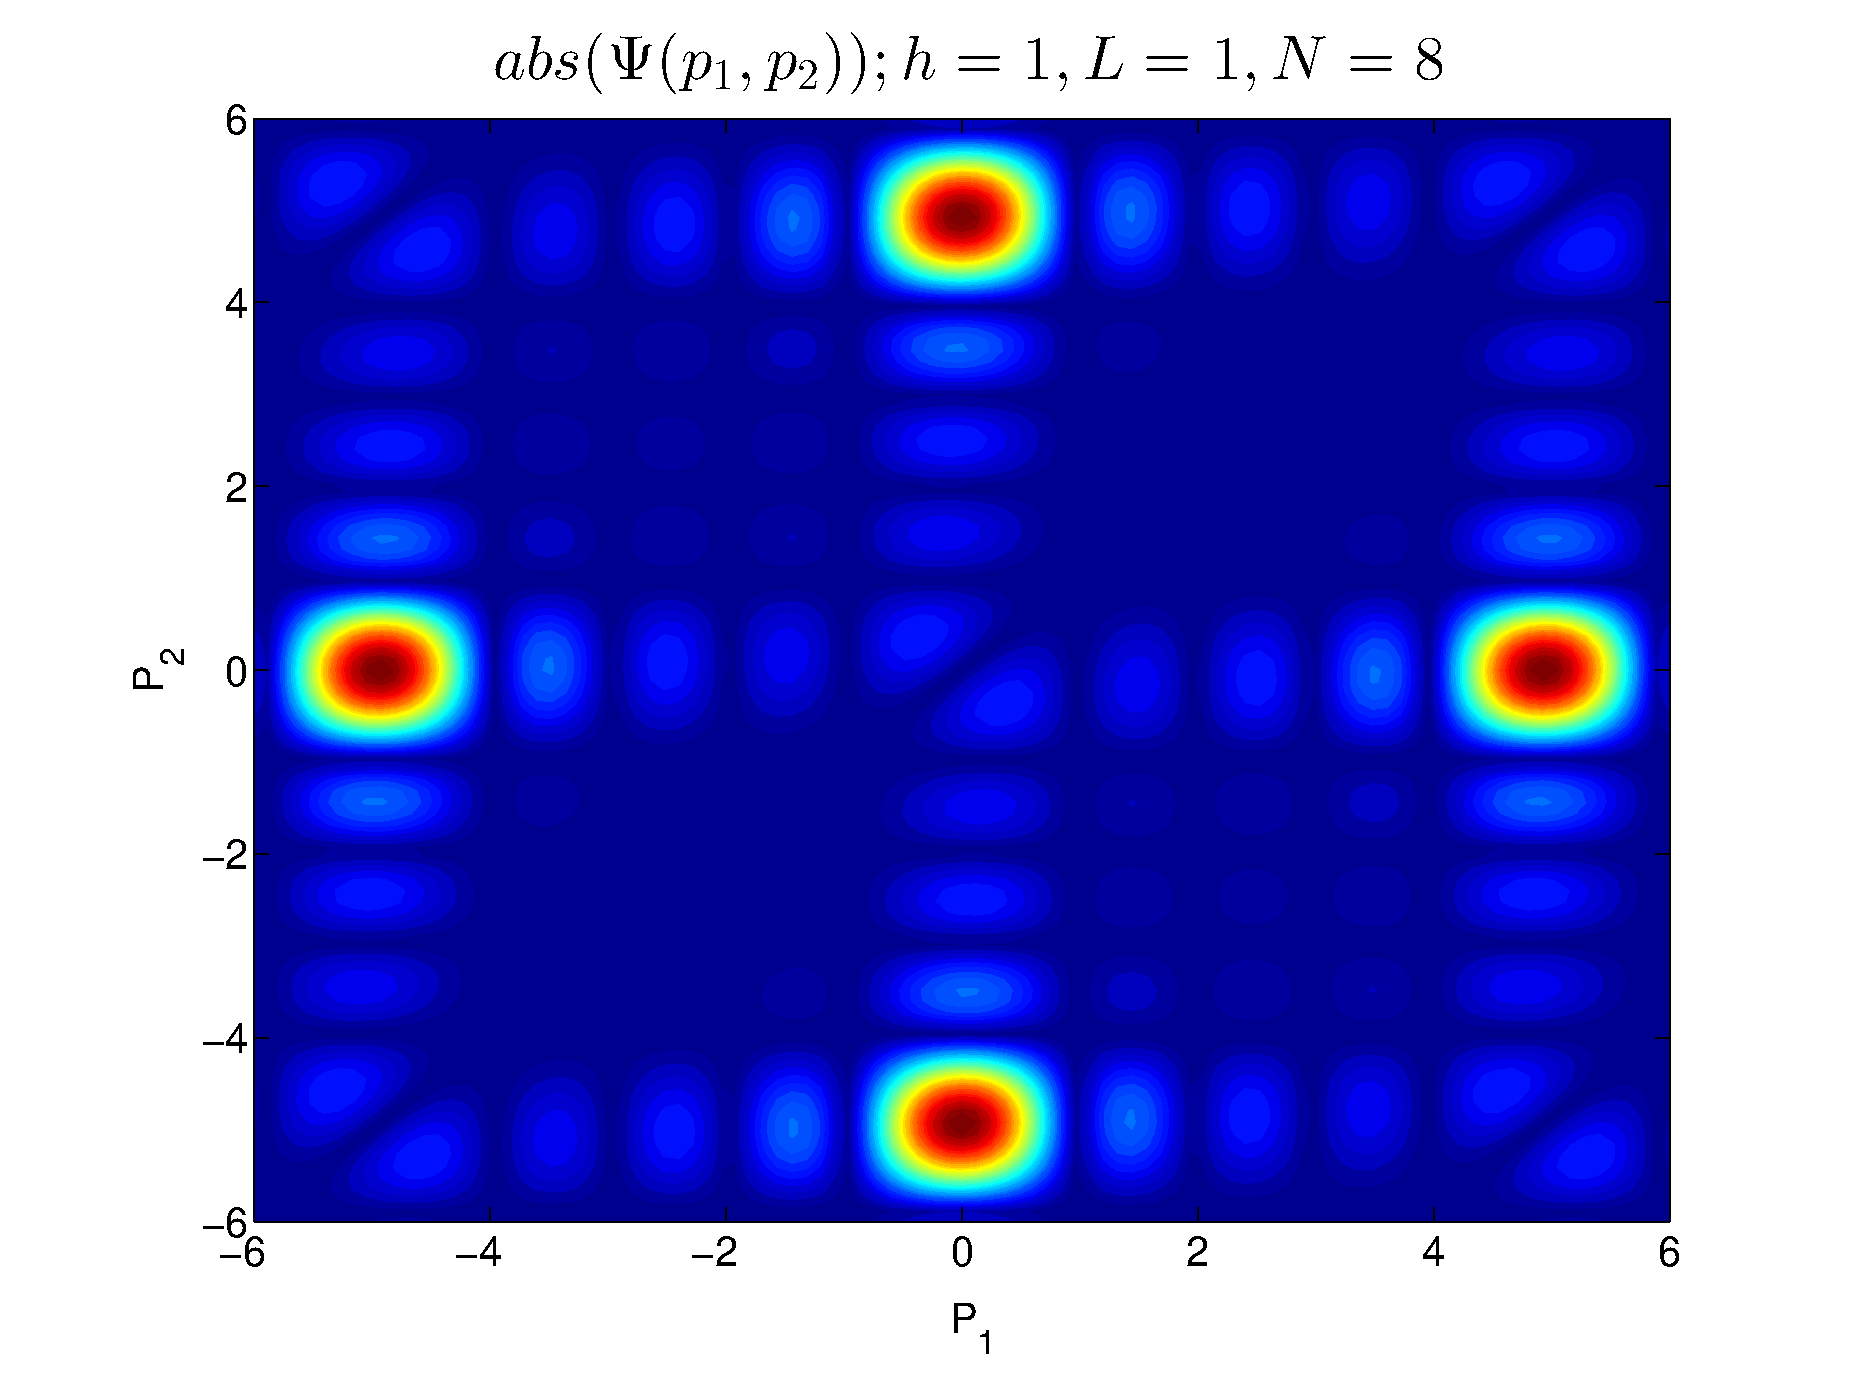
\includegraphics[width=6cm]{plots/entangledPsiN8}
\caption{Represents the expected histogram plotted after converting $(x_1,x_2) \to (p_1,p_2)$ using eqn \ref{eqn:measure}, for a fixed $\ket{\Psi_f}$ \label{fig:psiTilde}}
\end{figure}

\bibliography{Modular}

\end{document}
